% !TEX root = ./../main.tex
\chapter{Free energy calculations}
%Introduzione al lavoro svolto durante la tesi per quanto rigurda le matadinamiche

The preliminary metadynamics results from \cite{ourPaper} and summarized in section~\ref{sec:preliminaryMetadyn} of the charged ligand translocation across the membrane are made using the standard \martini \ac{FF} with a cut--off method for treating the electrostatic interactions. Unfortunately, as we have seen in chapter~\ref{sec:EmpiricalFF}, such method poorly describe the processes that involve the electrostatic interaction and hence it underestimates the energy barriers of the processes that involve the interaction between ions, water molecules and hydrophobic regions. Moreover the use of the standard \martini water model does not improve the energy barriers estimation.

The pathway to improve the model is the use of the \ac{PME} method to better describe the electrostatic interaction and the use of the \ac{PW} model to improve the behavior of the water solvent. For a comparison to be made, the idea, is to follow the procedure as in section~\ref{sec:preliminaryMetadyn} and, with metadynamics runs, try to estimate the energy barrier of the anchoring process with the use of the \ac{PME} alone and in combination with the \ac{PW} model. 

Preliminary, some tests about the use of the \ac{PME} method and the \ac{PW} model with a pure \ac{POPC} bilayer was performed. Then metadynamics runs for obtaining the \ac{FES} of the anchoring process involving both the striped (\ac{MUS}:\ac{OT} $1$:$1$) and the random (\ac{MUS}:\ac{OT} $1$:$1$) \acp{NP}, were performed with the use of the \ac{PME} alone and in combination with the \ac{PW} model. 
%In view of the results, then, as better described in the next Chapter, unbiased \ac{MD} runs with the use of \ac{PME} and \ac{PW} involving all the \ac{NP} configurations were performed in order to investigate a possible change in the kinematic of the all the \ac{NP}--membrane interaction process.

\section{Metadynamics: system set--up and issues}
%tentativi di convergenza con bound
The idea for a comparison to be made on the basis of free energy calculations is to obtain the \ac{FES} of the anchoring process of one charged ligand as described in section~\ref{sec:preliminaryMetadyn} using the different \ac{NP} configurations with the new \martini models. Then, in order to understand if this more sophisticated \ac{CG} models is suitable to better describe such process a comparison with an atomistic simulation\footnote{All the atomistic simulations and metadynamics runs are performed by Federica Simonelli in her PhD study} is necessary. In this way we can investigate if a more realist description can be obtained with a \ac{CG} model in order to use it for future applications.

To summarize briefly, the process that I will consider for the \ac{FES} estimation of the ligand anchoring is composed of two steps: the first, called forward process: from the hydrophobic state to one anchor state; the second, backward process: from the anchored state to the hydrophobic state again. 

\paragraph{\textbf{system set--up}} In all of my \ac{MD} runs the membrane bilayer is made of $256$ \ac{POPC} lipids per leaflet. I will consider both the striped (\ac{MUS}:\ac{OT} $1$:$1$) and the random (\ac{MUS}:\ac{OT} $1$:$1$) \acp{NP}. The simulation box is neutralized with $30$ counteracting Na$^+$ ions and filled by water. The initial configuration frames with the \ac{PW} are obtained using a python script that convert the standard \martini water to the \ac{PW} bead. Then an equilibration run with parameters as in the third column of table~(\ref{tab:inputParam}) is necessary to stabilize the system. For what concern the metadynamics input parameters, if not differently specified, they are summarized in table~(\ref{tab:metadynParam}).

\paragraph{\textbf{CV issues}} The \ac{CV} chosen to describe the anchor process is the $z$ component of the distance between the center of the charged bead and the \ac{COM} of the bilayer. Although it is a very intuitive and simple \ac{CV} and the pathway previously indicated, with the introduction of the \ac{PME}, and more accentuated with the \ac{PW} model, it suffers from some issues. When I perform the metadynamics runs with the \ac{PME} and the \ac{PW} model, in accordance with the atomistic model, it is observed that the anchored state is more stable than with the standard \martini models: the increase of the model accuracy make the interaction between the negatively charged bead and the positively charged choline group of the lipid heads of the opposite leaflet, stronger than with the standard \martini. Hence, like in figure~(), we observe that when metadynamics try to dis--anchor the charged bead in the backward process, it pull back the lipid heads slightly deforming the opposite leaflet of the bilayer. This results in a worse estimation of the \ac{CV}. Moreover, since the interaction with the lipid heads is stronger, the ligand tend to slightly pull down the \ac{NP} inside the bilayer, as shown in figure~(). Hence the movement of when the ligand is approaching the water phase of the opposite leaflet is not only due to the ligand itself but also because the \ac{COM} of the \ac{NP} tend to approach the center of the bilayer. Despite this can be an important molecular process, for now, in order for a comparison to be made, we do not want to sample the phase phase associated to the movement of the \ac{COM} of the \ac{NP} since it can lead to a worse estimation of the \ac{FES} associated to the anchoring process only. An other import issue as the simulation time increase and related to the previous, is the loss of ability by the \ac{CV} to well distinguish the two states, although the convergence has not yet reached. As we can see from figure~(\ref{fig:convTest}), this leads in an region of the \ac{CV} space in which the two states are overlapping. As confirmed with my unbiased runs, this issue leads in a underestimation of the forward wall because tend to lower the saddle point when the metadynamics is sampling the anchored state.
\begin{figure}[!ht]
	\centering
	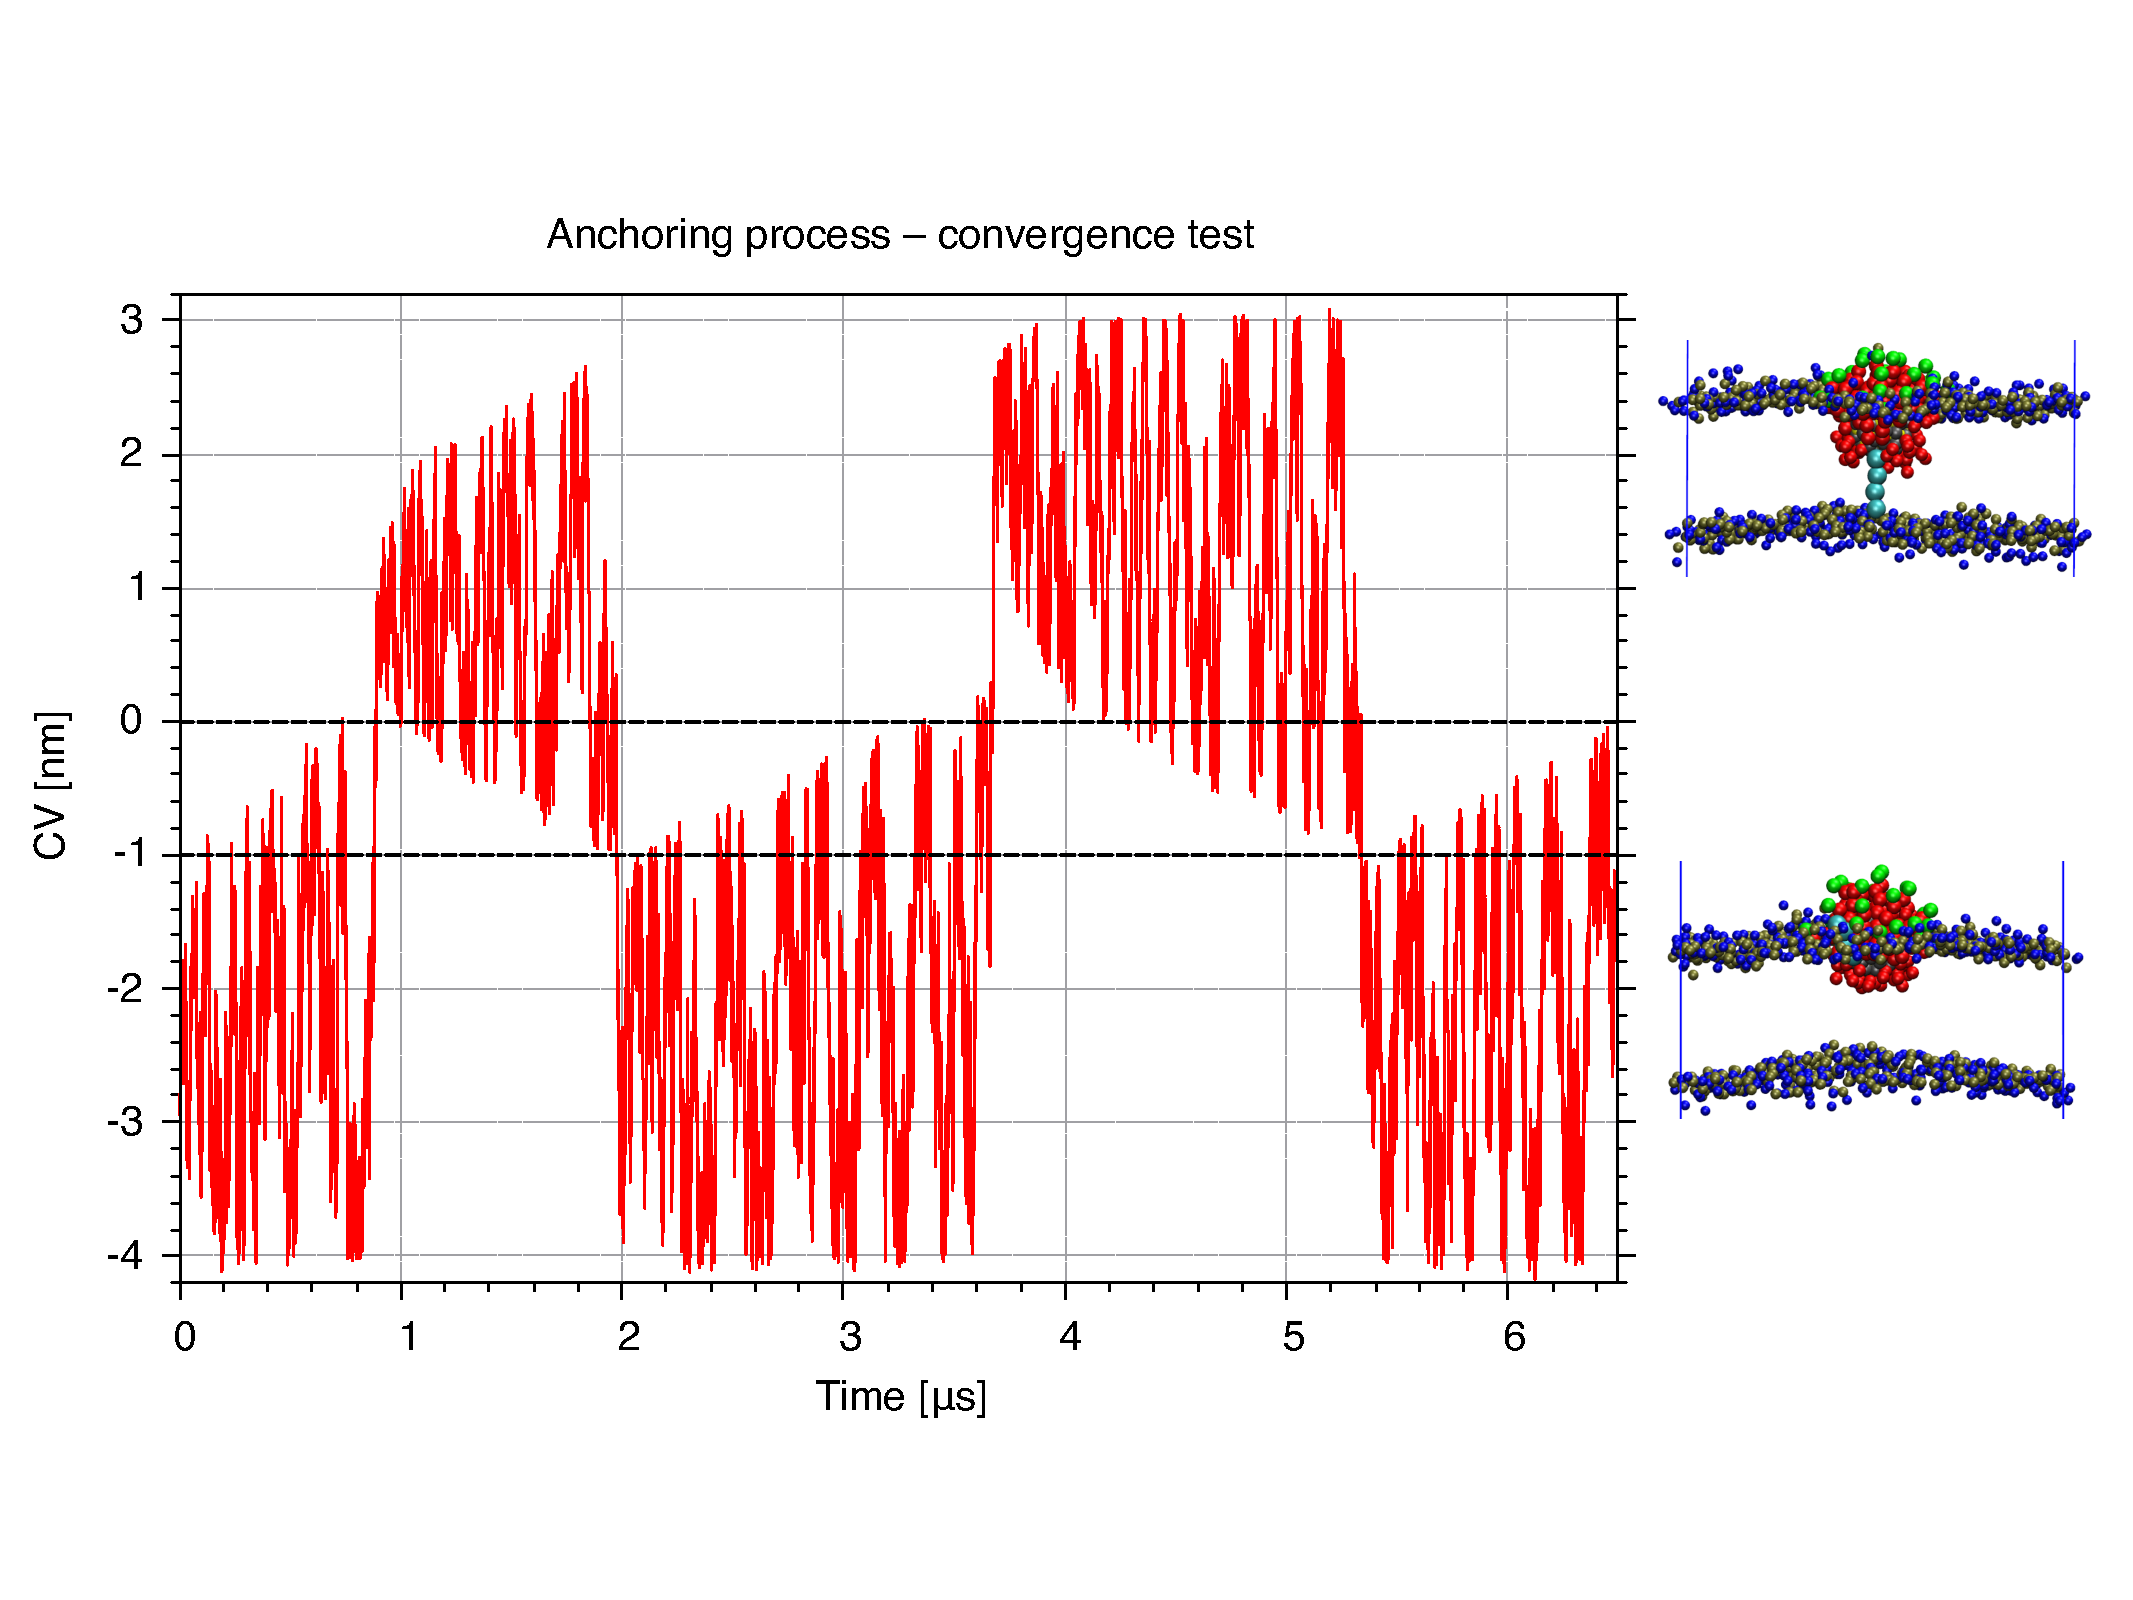
\includegraphics[width=0.95\textwidth]{./img/results/convTest}
	\caption{Convergence test for a metadynamics runs of a striped (\acs{MUS}:\acs{OT} $1$:$1$) \acs{NP}. The region of the \acs{CV} space inside the dashed lines is the overlapping region.}
	\label{fig:convTest}
\end{figure}

\paragraph{\textbf{convergence problems}} An other issues related to this process is the achievement of the convergence, essential in the \ac{FES} estimation. Our metadynamics runs have not reached the convergence, even in tens of microseconds of simulations, as we can see from figure~(\ref{fig:convTest}) from a $6.5$~$\mu$s test run trying to reach the convergence. This is prevalently due to the just described issues associated to the \ac{CV}. But also, in accordance with my unbiased simulations and the atomistic results, because the energy barriers associated to the two metastable state are much higher than what are estimated in \cite{ourPaper}, slowing down the dynamics. 

\paragraph{\textbf{worse estimation of the FES}} From the previous descriptions it is clear that following the procedure outlined in \cite{ourPaper} leads to a worse estimation of the \ac{FES} associated to the anchoring process. Using the same \ac{CV}, instead to try to estimate the whole \ac{FES}, we can try to estimate the energy wall associated to the forward process and, separately, the energy wall associated to the backward process. For the estimation of the energy wall of the forward process we need to start the metadynamics runs in the hydrophobic state and stop it when the ligand reach the anchored state. For the backward process we need to do the contrary: start the metadynamics from the anchored state and stop it when the ligand return to \ac{NP} leaflet.
%la usiamo per stimare la barriera di andata e ritorno

\section{Forward process}
Since the preliminary task of my thesis work, I have performed ten metadynamics runs starting at hydrophobic state for each of the following ``configurations'': striped (\ac{MUS}:\ac{OT} $1$:$1$) with \ac{PME}; striped (\ac{MUS}:\ac{OT} $1$:$1$) with \ac{PME} and \ac{PW}; random (\ac{MUS}:\ac{OT} $1$:$1$) with \ac{PME} and \ac{PW}. This runs are suitable for the estimation of the forward energy wall.
 
\subsection{Models comparison}
%striped models comparison (Standard, PME, PME & PW, Atomistico)
A comparison of the forward wall obtained for the striped (\ac{MUS}:\ac{OT} $1$:$1$) \ac{NP} with different models is shown in figure~(\ref{fig:forwardWall}). For the \ac{PME} and the \ac{PME}+\ac{PW} versions is shown an average over ten simulations each. For the STD version is shown an average over eight simulations. The atomistic version is obtained over an average of two simulations by Federica Simonelli. The error is estimate using the standard error as in the procedure described in section~\ref{sec:metadynamics}. As we can see, increasing the accuracy of the \ac{CG} model, the \ac{PW} model is approaching the atomistic results. Moreover, as we shall later, the order of magnitude of the energy barrier is consistence with my unbiased simulations in which for ten of microseconds no anchor process is observed, suggesting that the energy wall is much higher than what obtained in \cite{ourPaper}. 
\begin{figure}[h!t]
	\centering
	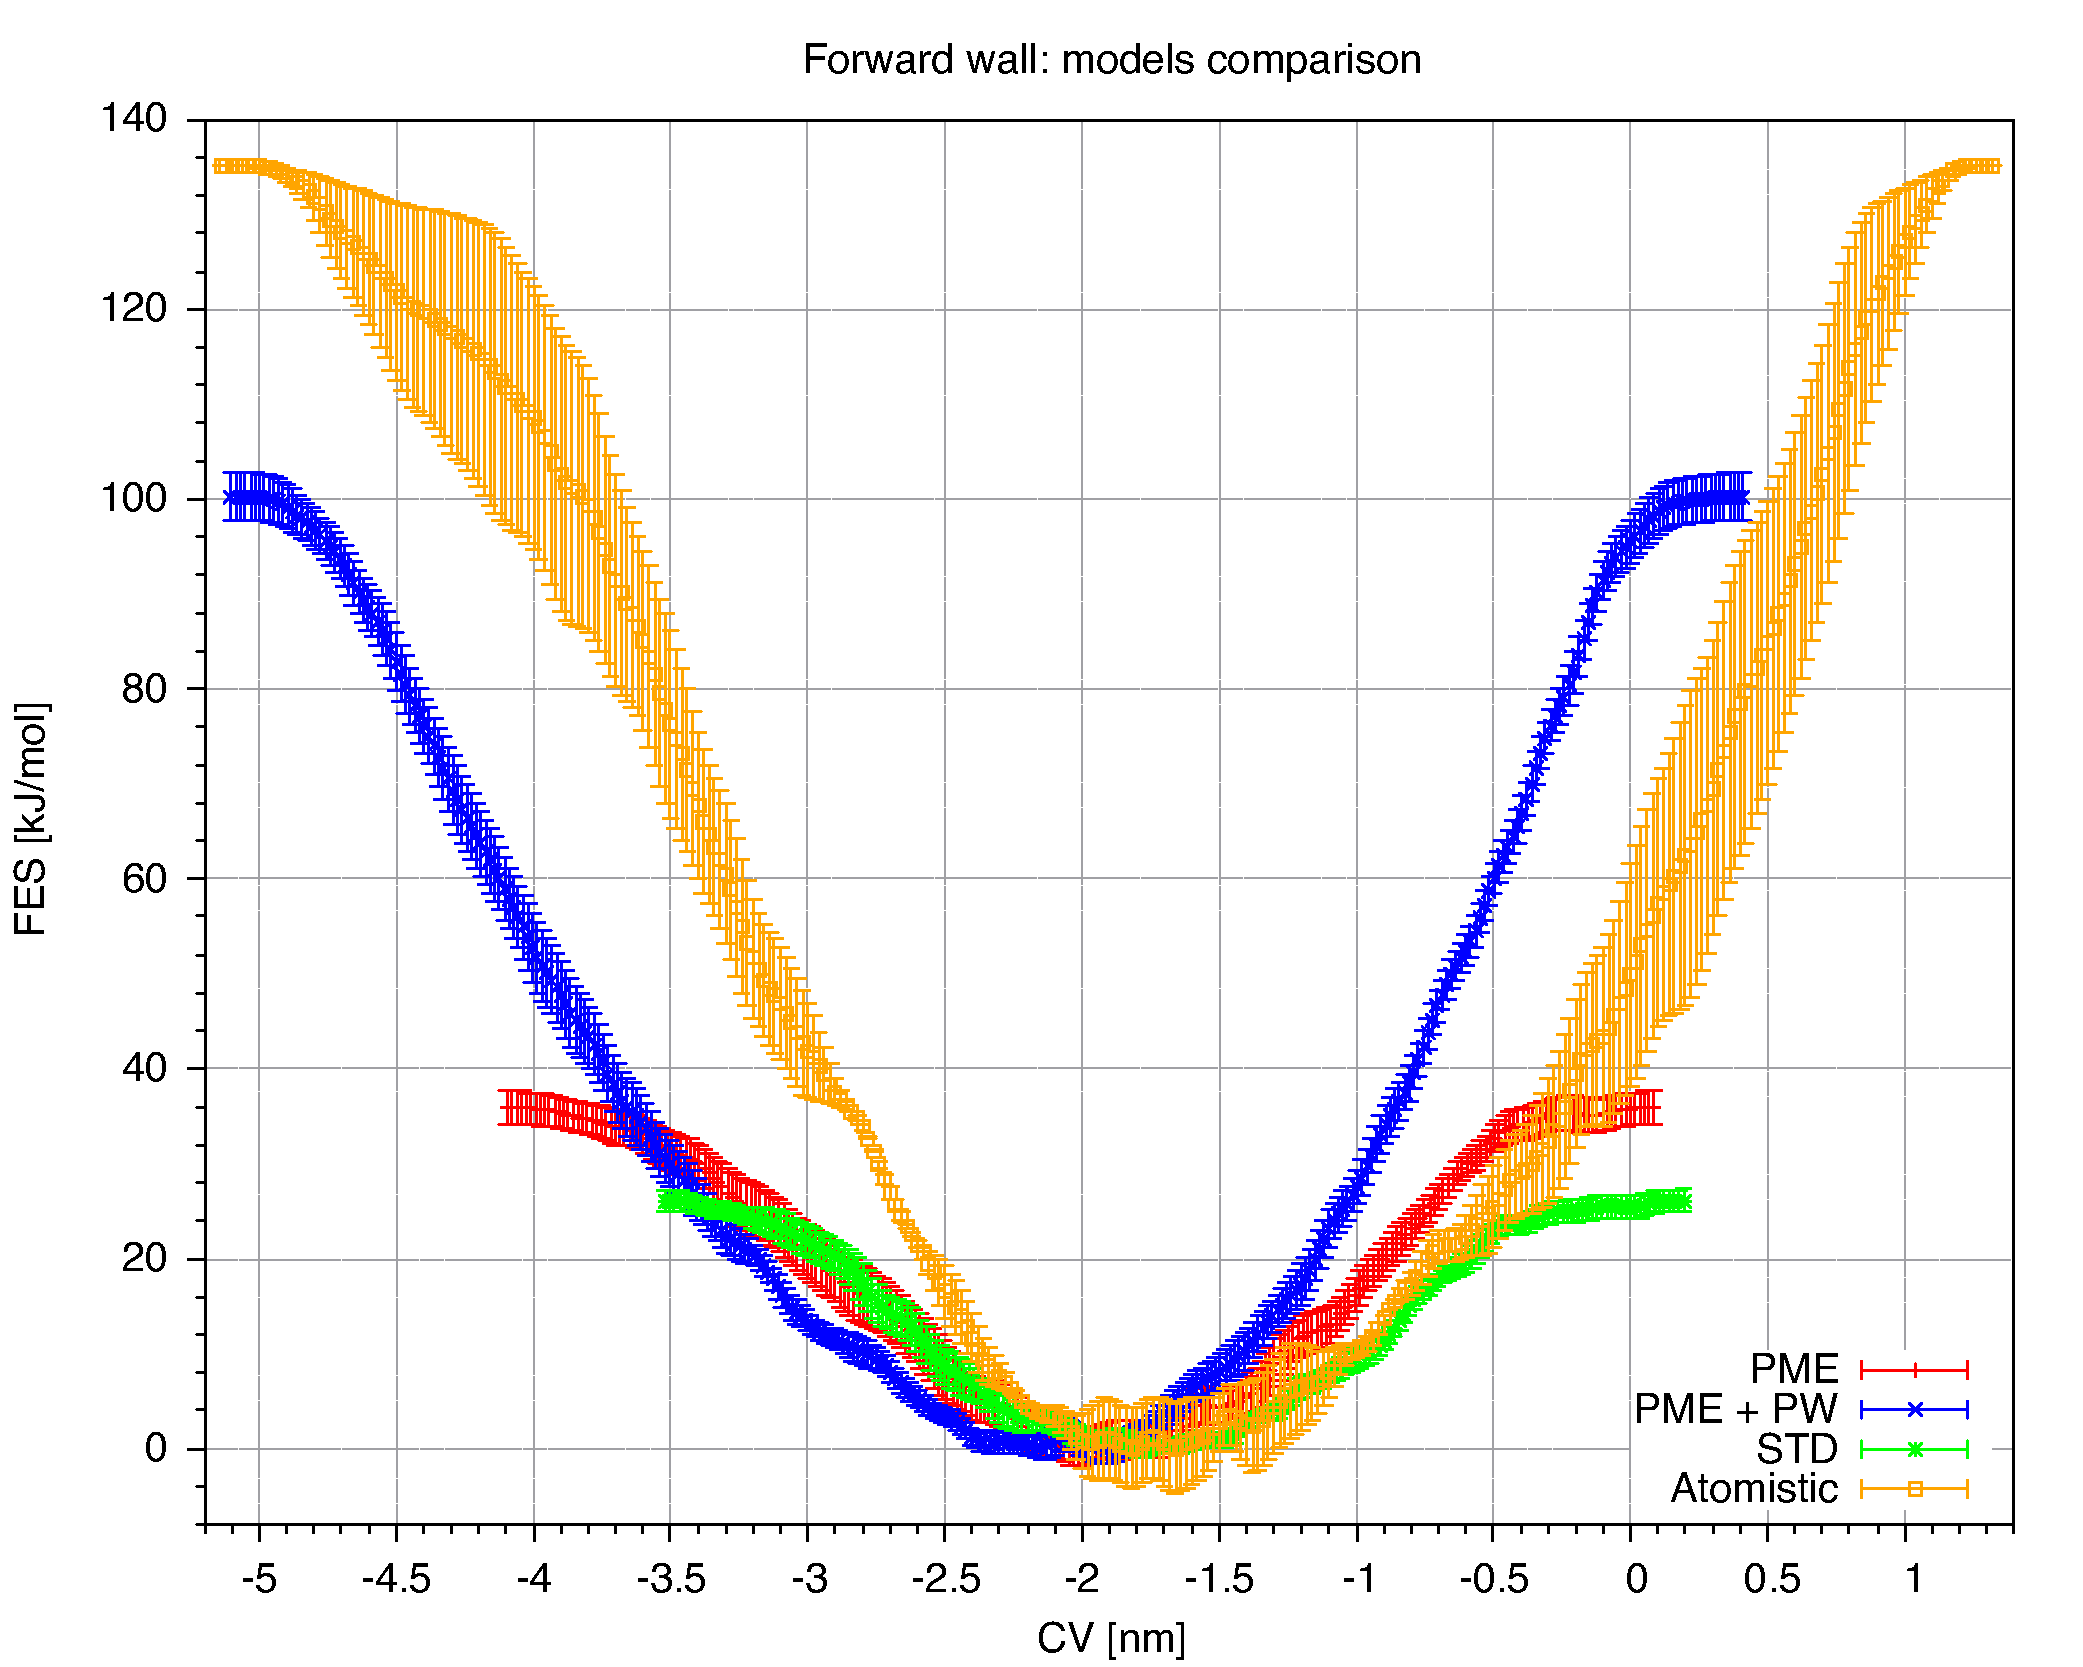
\includegraphics[width=0.9\textwidth]{./img/results/FESModelComparison/forwardWall}
	\caption{Model comparison of the forward wall.}
	\label{fig:forwardWall}
\end{figure}

\subsection{Striped and random comparison}
	%metadinamiche patched e random con PME e PW
The simulations allow for a comparison of the forward energy wall for both striped (\ac{MUS}:\ac{OT} $1$:$1$) and random (\ac{MUS}:\ac{OT} $1$:$1$) \acp{NP}. The comparison is shown in figure~(\ref{fig:forwardWallRP}). We can confirm the trend observed in \cite{ourPaper}: the striped (\ac{MUS}:\ac{OT} $1$:$1$) \ac{NP} has an higher energy wall for the hydrophobic to one anchor state transition than that for the random (\ac{MUS}:\ac{OT} $1$:$1$) \ac{NP}.
\begin{figure}[h!t]
	\centering
	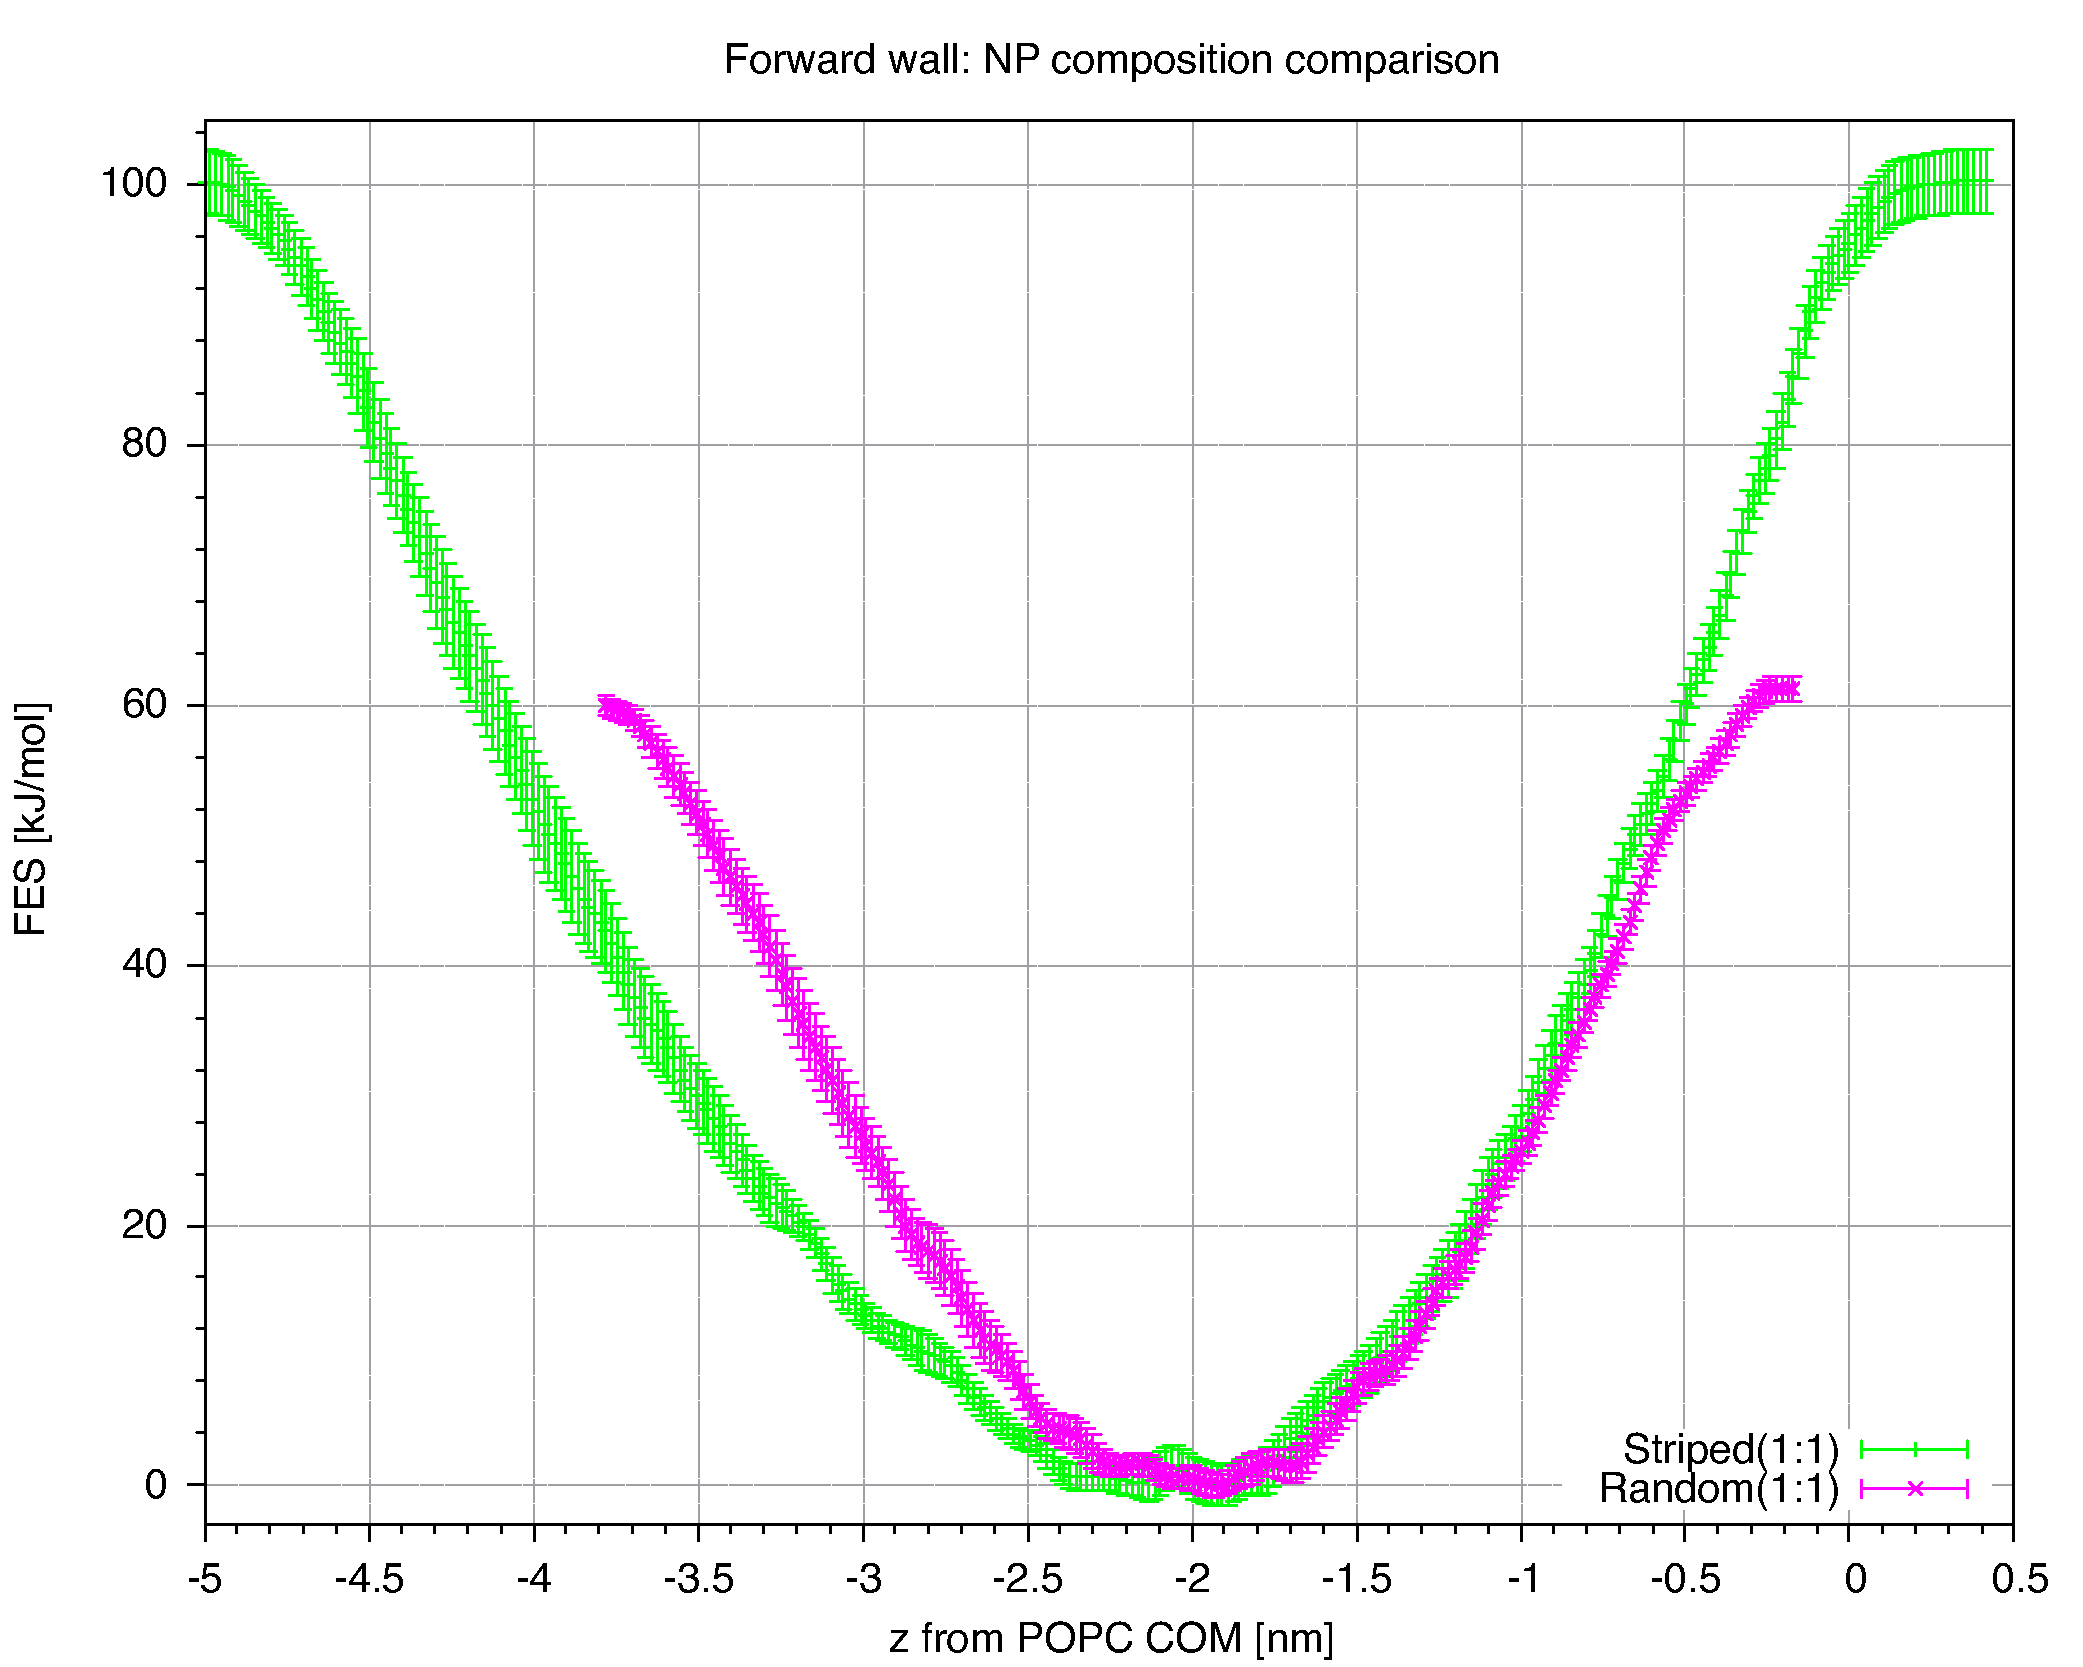
\includegraphics[width=0.9\textwidth]{./img/results/FESModelComparison/forwardWallRP}
	\caption{Forward energy wall in a comparison with the \ac{NP} at different ligand surface arrangements.}
	\label{fig:forwardWallRP}
\end{figure}
	
\section{Recrossing process: preliminary results}


\section{Discussion of the results}


% \paragraph{\textbf{ions translocation}} An important phenomenon mediated by the electrostatic interactions that is crucial for this thesis work is the lipid membrane ions translocation. In \cite{PW} the authors have computed the \ac{FES} of the translocation of Na$^+$ and Cl$^-$ ions\footnote{The \martini model for Na$^+$ and Cl$^-$ associates the ion plus the hydration shell to a bead of type Qd positively charged and Qa negatively charged, respectively.} across a \acs{DPPC} membrane using umbrella sampling and the \ac{WHAM} with the standard \martini \ac{FF}, adding the \ac{PW} and adding together \ac{PW} and \ac{PME}. The height of the barriers are summarized in table~(\ref{tab:ionTranslocation}). The same \ac{FES} for a \acs{DMPC} membrane was calculated by Khavrutskii \etal\, \cite{atomisticTranslocation} with an atomistic \ac{FF}. Since the \martini model for the \acs{DPPC} lipid also model the \acs{DMPC} lipid a comparison can be made and it is shown in table~(\ref{tab:ionTranslocation}). As one can see, from left to right, increasing the loyalty of the treatment of the electrostatic interaction the \martini \ac{FF} approach the results of the atomistic \ac{FF}. Moreover in \cite{PW}, in accordance with the atomistic results in \cite{atomisticTranslocation}, for small cross membrane ions imbalance and only with the use of the \ac{PW} model and the \ac{PME} method, they observe some ion leakage without pore formation but still mediated by a water defect inside the membrane, called \textit{water finger} that help the ions to cross the hydrophobic region of the membrane. We remark that, these kind of phenomena, are totally absent using the standard \martini \ac{FF}. Hence, as already outlined, the importance to use a better treatment of the electrostatic interaction and a better model for water solvent.
% \begin{table}[h!t]
% 	\centering
% 	\begin{tabular}{lcccc}
% 		\toprule
% 		\,		& Standard & \acs{PW} & \acs{PW} \& \acs{PME} & Atomistic	\\ \toprule
% 		Na$^+$	& 68.0	   & 67.6	  & 78.6					& 91.7 		\\ \midrule
% 		Cl$^-$	& 69.2	   & 70.4	  & 99.0					& 98.8		\\ \bottomrule
% 	\end{tabular}
% 	\caption{Height of the energy barrier (in kJ/mol) for Na$^+$ and Cl$^-$ translocation across a bilayer. The \martini results are based on a \acs{DPPC} membrane and are taken from \cite{PW} while the atomistic are based on a \acs{DMPC} membrane and are taken from \cite{atomisticTranslocation}.}
% 	\label{tab:ionTranslocation}
% \end{table}
